In this section we want to derive the result (\ref{eq:expansion_coefficients_debye_BCF_SBM}), that is
coefficients $g_j$ and $w_j$ such that the bath correlation function
\begin{equation*}
    \alpha(\tau) = \frac{1}{\pi} \int_0^\infty S(\omega)
    \left[
        \coth\left(\frac{\omega}{2T}\right)\cos(\omega\tau)-i\sin(\omega\tau)
    \right]\text{d}\omega
    = \int_0^\infty I(\omega,\tau)\text{d}\omega
\end{equation*}
with the \textit{Debye spectral density}
\begin{equation*}
    S(\omega) = \eta \frac{\omega\gamma}{\omega^2+\gamma^2}
\end{equation*}
can be approximated as a sum of exponentials
\begin{equation*}
    \alpha(\tau) \approx \sum_{j=0}^{N_{BCF}}g_je^{-\omega_j\tau}.
\end{equation*}
To compute the expansion coefficients $g_j$ and $\omega_j$, we will use a \textit{Matsubara expansion}.
First we note that the integrand $I(\omega, \tau)$ is symmetric with respect to $\omega$,
$I(-\omega, \tau) = I(\omega, \tau)$. Hence, we can extend the integral over the negative real axis:
\begin{equation*}
    \alpha(\tau) = \frac{1}{2} \int_{-\infty}^\infty I(\omega,\tau)\text{d}\omega.
\end{equation*}
We further split the integral into a real and an imaginary part $\alpha(\tau) = a(\tau) + i b(\tau)$, where
\begin{equation*}
    a(\tau) = \frac{1}{2\pi}\int_{-\infty}^\infty S(w)\coth\left(
        \frac{\omega}{2T}
    \right) \cos(\omega\tau) \text{d}\omega
\end{equation*}
and
\begin{equation*}
    b(\tau) = -\frac{1}{2\pi}\int_{-\infty}^\infty S(w)\sin(\omega\tau)\text{d}\omega.
\end{equation*}
Expanding the sine and cosine in terms of exponentials and using the antisymmetry of the
hyperbolic cotangent and the Debye spectral density, we can write
\begin{equation*}
    a(\tau) = \frac{1}{2\pi}\int_{-\infty}^\infty S(\omega)\coth\left(
        \frac{\omega}{2T}
    \right)e^{i\omega\tau},
\end{equation*}
\begin{equation*}
    b(\tau) = -\frac{1}{2\pi i}\int_{-\infty}^\infty S(\omega)e^{i\omega\tau}.
\end{equation*}
\begin{figure}[h]
    \centering
    \label[figure]{fig:line_integral_matsubara_expansion}
    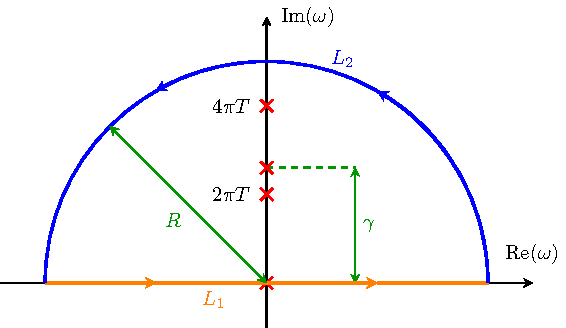
\includegraphics{tikz/matsubara_expansion/matsubara_expansion.pdf}
    \caption[short]{In this figure, the line integral for computing the expansion of the bath correlation function is shown.}
\end{figure}
To solve the integrals, we will use the residual theorem. Consider the line integral in figure \ref{fig:line_integral_matsubara_expansion}. 
Because of the exponential $e^{i\omega\tau}$, the contribution
along $L_2$ vanishes as we take the limit $R\rightarrow\infty$. This leaves us with
\begin{equation*}
    \begin{split}
        a(\tau) &= \frac{1}{2\pi}\oint_\xi S(\omega)\coth\left(
        \frac{\omega}{2T}
        \right)e^{i\omega\tau} \text{d}\omega = i\sum_{\{\omega_j\}}\Residue\left(
            S(\omega)\coth\left(
                \frac{\omega}{2T}
            \right); \omega_j
        \right)e^{i\omega_j\tau}\\
        &= i\sum_{\{\omega_j^\prime\}} \Residue\left(
            S(\omega); \omega_j^\prime
            \right) \coth\left(
                \frac{\omega_j^\prime}{2T}
            \right)e^{i\omega_j^\prime\tau} + 
            i\sum_{\{\omega_j^{\prime\prime}\}} \Residue\left(
            \coth\left(
                \frac{\omega}{2T}
            \right); \omega_j^{\prime\prime}
            \right) S(\omega_j^{\prime\prime}) e^{i\omega_j^{\prime\prime}\tau}, \\
        b(\tau) =& -\frac{1}{2\pi} \oint_\xi S(\omega) e^{i\omega\tau} \text{d}\omega =
    -\sum_{\{\omega_j^\prime\}} \Residue\left(
            S(\omega); \omega_j^\prime
            \right) e^{i\omega_j^\prime\tau},
    \end{split}
\end{equation*}
where $\omega_j$ are the poles of $S(\omega)\coth\left(\frac{\omega}{2T}\right)$,
$\omega_j^\prime$ the poles of $S(\omega)$, $\omega_j^{\prime\prime}$ the poles of
$\coth\left(\frac{\omega}{2T}\right)$, and we used the residue theorem. We also
assumed $\omega_j^\prime \neq \omega_b^{\prime\prime}$ for all $a, b$, which is the case for almost all $\gamma$ and $T$. Next, we need to compute
the poles and residues. The Debye spectral density has simple poles at $\omega_j^\prime=\pm i\gamma$,
with residuals
\begin{equation*}
    \Residue\left(S(\omega);\pm i\gamma\right) = \lim_{\omega\rightarrow i\gamma}(\omega\mp i\gamma)S(\omega) = \frac{\eta\gamma}{2}.
\end{equation*}
The poles of the hyperbolic cotangent $\coth\left(\frac{\omega}{2T}\right)$ lie on the imaginary axis, $\omega_j^{\prime\prime} = 2\pi iTa$ with $a\in\mathbb{Z}$,
and are again simple poles with residuals
\begin{equation*}
    \Residue\left(\coth\left(\frac{\omega}{2T}\right);2\pi iTj\right) =
    \lim_{\omega\rightarrow 2?pi iTj} (\omega-2\pi iTj) \coth\left(
        \frac{\omega}{2T}
    \right) = \lim_{\lambda\rightarrow 0} 2T\lambda\coth(\lambda) = 2T,
\end{equation*}
where we used the identities $\coth(x+i\pi n) = \coth(x)$ for $n\in\mathbb{Z}$ and $\lim_{x\rightarrow
0}x\coth(x)=1$.
\\
With this, we are now equipped to solve the integrals:
\begin{equation*}
    b(\tau) = -\frac{\eta\gamma}{2} e^{-\gamma\tau},
\end{equation*}
\begin{equation*}
    a(\tau) = i\frac{\eta\gamma}{2}\coth\left(
        \frac{i\gamma}{2T}
    \right)e^{-\gamma T} + i\sum_{j=1}^{\infty}2T\,S(2\pi iTj)\,e^{-2\pi Tj\tau}.
\end{equation*}
Putting the results together, we can write
\begin{equation*}
    \alpha(\tau) = a(\tau) + ib(\tau) = \sum_{j=0}^{\infty} g_j e^{-\omega_j\tau}
\end{equation*}
with the coefficients (\ref{eq:expansion_coefficients_debye_BCF_SBM}).
The result is similar to the one obtained in \cite{Qiang:2009} (up to a different normalization).